\documentclass[12pt]{article}
\usepackage[utf8]{inputenc}
\usepackage[russian]{babel}
\usepackage{amsmath}
\usepackage{amssymb}
\usepackage{geometry}
\usepackage{graphicx}
\geometry{a4paper, margin=1in}
\usepackage{listings}
\usepackage{xcolor}

\lstset{
  language=C++,                % Язык программирования
  basicstyle=\ttfamily\small,  % Шрифт и размер текста
  keywordstyle=\color{blue},   % Цвет ключевых слов
  commentstyle=\color{gray},   % Цвет комментариев
  stringstyle=\color{red},     % Цвет строк
  numbers=left,                % Нумерация строк слева
  numberstyle=\tiny\color{gray}, % Стиль номеров строк
  stepnumber=1,                % Интервал нумерации строк
  breaklines=true,             % Перенос длинных строк
  frame=single,                % Рамка вокруг кода
}

\title{Отчёт по расчётной работе по дисциплине ПиОИвИС}
\author{}
\date{}


\begin{document}

\maketitle

\begin{center}
\section*{Графы}
\end{center}

\subsection*{Задача}
Научится работать и проводить различные операции с графами.

\subsection*{Цель}
Найти объединение множества неориентированных графов

\subsection*{Вариант}
4.8 мc

\section*{Определения}

\begin{itemize}
    \item \textbf{Граф} —  математическая абстракция реальной системы любой природы, объекты которой обладают парными связями. Граф как математический объект есть совокупность двух множеств — множества самих объектов, называемого множеством вершин, и множества их парных связей, называемого множеством рёбер. Элемент множества рёбер есть пара элементов множества вершин.
    
    
    \item \textbf{Неориентрованный граф} — это граф у которого рёбра не указывают направление. Это значит, что из любой вершины можно попасть в любую точку графа.
    
    
     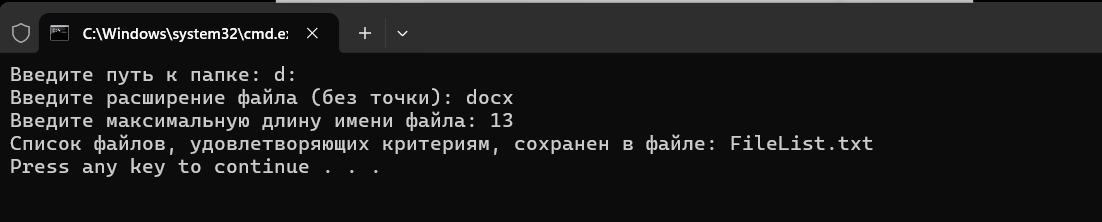
\includegraphics[width=0.7\textwidth, height=5cm, keepaspectratio]{1.png}
     
    \item \textbf{Сме́жность} — непосредственная близость, примыкание. В теории графов смежность вершин соответствует наличию ребра между ними.
    
    \item \textbf{Матрица смежности} - это вид представления графа в виде матрицы, когда пересечение столбцов и строк задаёт дуги.
    
        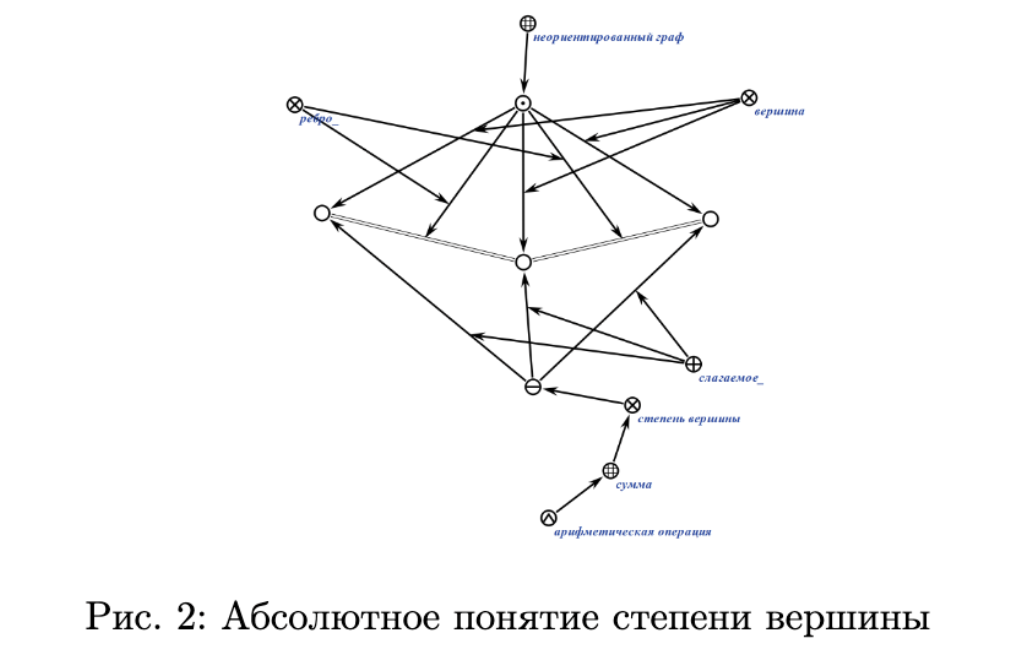
\includegraphics[width=0.8\textwidth, height=10cm, keepaspectratio]{2.jpeg}
        
\end{itemize}

\section*{Алгоритм}
\begin{enumerate}
    \item Создаётся пустой граф unionGraph для объединения графов.
    \item Ввод первого графа.
    \item Ввод второго графа.
    \item Подгон размера матриц с помощью resizeMatrix.
    \item Объединение графов функцией UnionGraphs() .
    \item Считать первый и второй граф из файла graph1.txt и graph2.txt с помощью readGraphFromFile() и объединить его с unionGraph.
    \item Используя displayGraph() вывести итоговую матрицу смежности объединенного графа.
    
\end{enumerate}

\section*{Пример работы кода}
 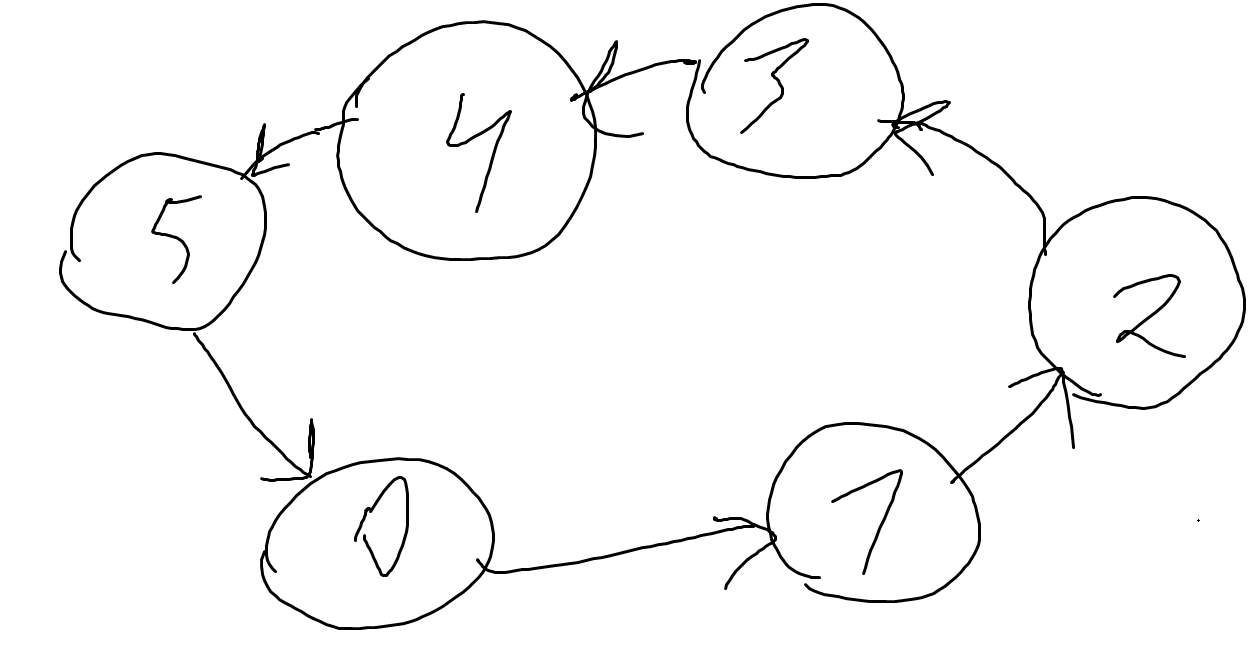
\includegraphics[width=0.5\textwidth, height=10cm, keepaspectratio]{3.jpg}
 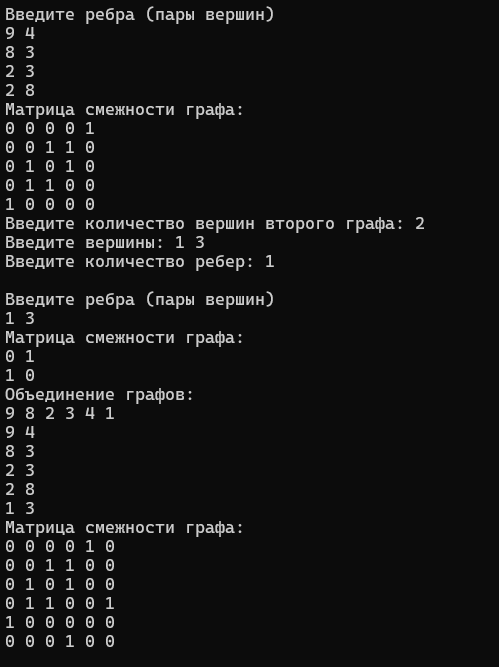
\includegraphics[width=0.5\textwidth, height=10cm, keepaspectratio]{4.jpg}
 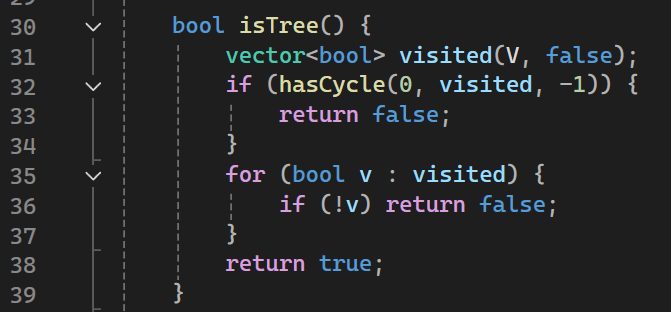
\includegraphics[width=0.5\textwidth, height=10cm, keepaspectratio]{5.jpg}
 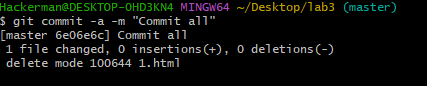
\includegraphics[width=0.5\textwidth, height=10cm, keepaspectratio]{6.jpg}
 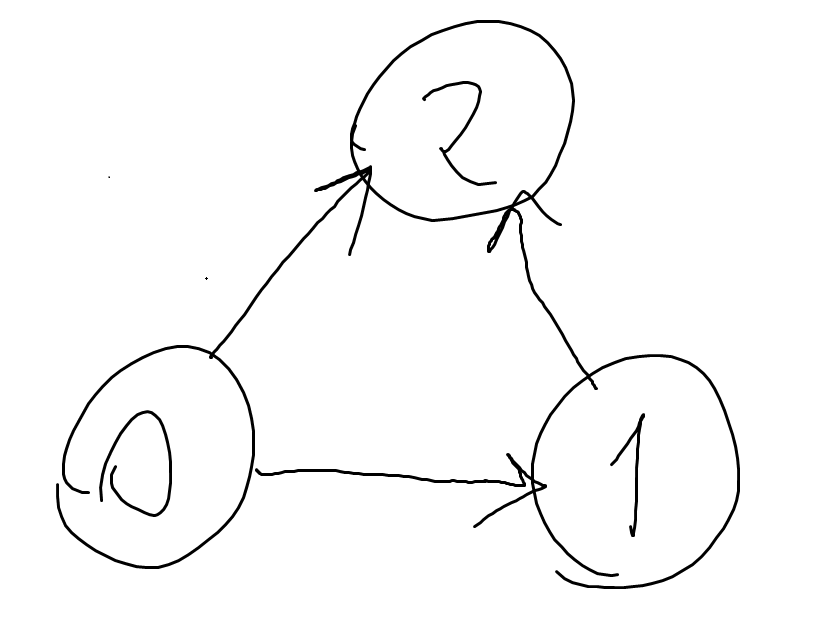
\includegraphics[width=0.5\textwidth, height=10cm, keepaspectratio]{7.jpg}
\section*{Вывод}

В результате выполнения данной работы были получены следующие практические навыки:

\begin{itemize}
    \item Изучены основы теории графов.
    \item Изучены способы представления графов.
    \item Изучены базовые алгоритмы для работы с графами.
\end{itemize}

\section*{Источники}
\begin{itemize}
\item https://www.geeksforgeeks.org/what-is-unidrected-graph-undirected-graph-meaning/
\item https://habr.com/ru/articles/564594/
\item https://en.wikipedia.org/wiki/Graph_theory
\end{itemize}
\end{document}